\documentclass{report}
\usepackage{fullpage}
\usepackage{graphicx}
\begin{document}
\title{Savant Genome Browser: User Manual}
\maketitle

\setlength{\parindent}{0pt} 
\setlength{\parskip}{2ex}

Author: Marc Fiume \\
Contact: savant@cs.toronto.edu \\
Website: http://compbio.cs.toronto.edu/savant/ \\
\\
This document applies to Savant version 1.02\\

\newpage

\tableofcontents

\newpage

\chapter{Introduction}

\section{What is Savant?}

Savant stands for "Sequence Annotation Visualization and Analysis Tool". In other words, Savant is a program for visualizing and analyzing genomics data. It was designed to run quickly and efficiently on conventional desktop or laptop computers.

\section{Who should use Savant?}

Savant makes visualization and analysis of genomics data very efficient. If you use genome browsers like UCSC or IGV or if you are a biologist or bioinformatician who works with genomics data, you should try Savant. 

\chapter{Formatting and Loading Data}

Savant supports a number file formats. These files are specially formatted before use to ensure speedy data retrieval. To learn how to directly output Savant formatted files, see the {\bf Developer's Guide} downloadable from the Savant website.

\section{Supported File Formats}

\subsection{Standard File Formats}

Savant supports the following standard file formats:

\begin{table}[ht] 
\caption{Supported File Formats}  
\begin{tabular*}{6in}{ l l }  
\hline                      
Format & Description \\
\hline                    
FASTA & for representing nucleotide sequences.  \\
BED & an alternative to GFF format. \\
GFF* & for genes and other localized features. \\   
SAM / BAM & for nucleotide  sequence alignments. \\
WIG & for continuous-valued data in track format. \\      
\hline     
\end{tabular*} 
\end{table} 

*Partial support.

\subsection{Non-standard (aka Generic) File Formats}

Savant also supports simple file formats for point, interval, and continuous annotations. Files in so-called "generic" format are tab-delimited and have the following fields on each line:

\begin{itemize}
\item Point: [int: position] [string: annotation]
\item Interval: [int: start position] [int: end position] [string: annotation]
\item Continuous*: [int/float: value]
\end{itemize}

*Note that for continuous files, the position at which the annotation applies is implicit in the line number. That is, the value on the ith row of a generic continuous file represents the value for position i on the genome. \\

Generic files can typically be generated easily with moderate knowledge of shell scripting.  

\section{Downloading Data}

A number of common annotations (e.g. sequence and gene) for the human genome have been formatted and hosted on the Savant website at http://compbio.cs.toronto.edu/savant/data.html.

Genomic annotations are also available from other databases. Downloading and formatting data from these and other popular data sources is encouraged:

\begin{itemize}
\item UCSC: http://genome.ucsc.edu/
\item 1000 Genomes Project: http://www.1000genomes.org
\item NCBI: http://www.ncbi.nlm.nih.gov/
\item EBI: http://www.ebi.ac.uk/
\end{itemize}

\section{Using the Format Dialog}

\label{usingformatdialog}

The Format Dialog can be used to format text files (e.g. ones downloaded from the various data sources listed above) for use with Savant. \\

The Format Dialog can be opened by choosing File \textgreater Format. \\

\begin{figure*}[!h]
\begin{center}
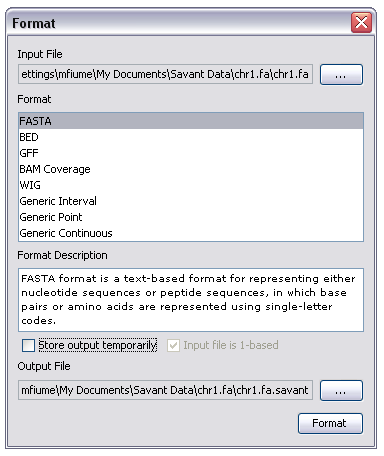
\includegraphics[type=png,ext=.png,read=.png,height=6cm]{images/formatdialog}
\caption{The Format Dialog.}
\label{formatdialog}
\end{center}
\end{figure*}

Components of the Format Dialog (see Figure \ref{formatdialog}):
\begin{itemize}
\item Input file: the text file to be formatted
\item Format: the format of the input file
\item Input is 1-based: whether or not the input file's positional annotations start at 0 or 1
\item Output file: the output file to be produced which can subsequently be loaded into Savant
\end{itemize}

\section{Loading Tracks}

A track is an individual data set (hence, tracks and data may be used interchangeably hereafter).

Files formatted for use with Savant typically have the ".savant" extension (BAM files are exceptions, which have ".bam" extensions). There may be other files created by the formatter with, for example, other extensions such as ".savant.index". It is essential that these accompanying files remain in the same folder as the .savant files. Otherwise, the files aren't likely to load properly.

\subsection{Track loading prerequisites}

\begin{enumerate}
\item Files must be formatted for use with Savant. For help with formatting files, please see Section \ref{usingformatdialog}. If you are unsure whether or not your file is formatted, you can try to load it and Savant will prompt for formatting if it does not appear to have been formatted.
\item A genome must be specified.\\
Option 1 : Loading a genome sequence from file -- A formatted genome sequence file is loaded by pressing the Genome button or by clicking File \textgreater Load \textgreater Genome and choosing "Load From File". This option loads the genome sequence as a track.\\
Option 2 : Specifying the genome's without providing a sequence -- A genome is specified without a sequence by pressing the Genome button or by clicking File \textgreater Load \textgreater Genome and choosing "Specify Length"; subsequently one can either choose from a list of common genome assemblies or specify a length.
\end{enumerate}

\subsection{Loading a Track}

A track is loaded by pressing the Track button or by clicking File \textgreater Load \textgreater Track and using the File Chooser Dialog to open the appropriate file.

\chapter{Navigation}

Navigation refers to changing the region of the genome which is viewed by the browser. A user can navigate by either interacting with the user interface (in particular, with the Navigation Toolbar located at the top of the interface) or by using the appropriate keyboard and mouse shortcuts.

\section{Navigation Toolbar}

\begin{figure*}[!h]
\begin{center}
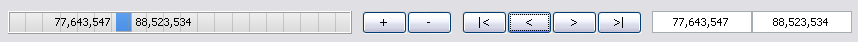
\includegraphics[type=png,ext=.png,read=.png,width=16cm]{images/rangecontrolpanel}
\caption{The Navigation Toolbar, found at the top of the Savant UI.}
\label{rangecontrolpanel}
\end{center}
\end{figure*}

Components of the Navigation Toolbar from left to right are described below in turn.

\subsection{Range Selection Panel}

The Range Selection Panel displays the current displayed region in the context of the genome. Users can select a new range by clicking and dragging within the panel.

\subsection{Zooming}

The zoom buttons allow the user to zoom in and out with respect to the current range. 

\subsection{Panning}

The pan buttons allow the user to shift the range to the left and to the right (including to the beginning of the genome and to the end of the genome). 

\subsection{Seeking to specific range}

Textboxes are afforded for the user to enter precisely the range to be displayed. The range will be updated using the values entered in the textboxes when the user presses the Enter/Return key while one of the textboxes has focus.

\section{Mouse and Keyboard Shortcuts}

Navigation can be done very quickly using a number of mouse and keyboard shortcuts described in the tables below.

\begin{table}[h] 
\caption{Navigation using the keyboard}  
\begin{tabular*}{6in}{ l l }  
\hline                      
Keys & Action \\
\hline                    
CTRL/CMD+LEFT & pan left  \\
CTRL/CMD+RIGHT & pan right \\ 
CTRL/CMD+UP & zoom in \\     
CTRL/CMD+DOWN & zoom out \\  
\hline     
\end{tabular*} 
\end{table} 

\begin{table}[h] 
\caption{Navigation using the mouse}  
\begin{tabular*}{6in}{ l l }  
\hline                      
Keys & Action \\
\hline            
Click and drag left/right & pan left/right  \\
CTRL/CMD + Scroll up/down & pan left/right  \\
CTRL/CMD + Click and drag  & zoom in on selected region  \\
Scroll up/down & zoom in/out  \\
\hline     
\end{tabular*} 
\end{table} 

\section{Other Useful Shortcuts}

Range changes can be undone and redone using the commands in the following table. Another option to save history is by clicking the "Record" button in the Bookmarks module, which keeps track of range viewed. This history can subsequently be saved for reviewing. See the Bookmarks section for more details.

\begin{table}[h] 
\caption{Undoing and Redoing Range Changes}  
\begin{tabular*}{6in}{ l l }  
\hline                      
Keys & Action \\
\hline                    
CTRL/CMD+Z & undo range change  \\
CTRL/CMD+Y & redo range change \\ 
\hline     
\end{tabular*} 
\end{table} 

\chapter{Visualization}

Savant retrieves and renders data every time a range change is requested by the user. Together, these processes happen nearly instantaneously so as to confer seamless navigation around the genome. The renderer for each track is adaptive to both the display mode and the length of the viewed region chosen by the user.

\section{Changing visualization mode}

Particular data types can be displayed in different modes. For example, interval annotations can be squished together on a single line or packed neatly so that none overlap (mimicking the squish and pack modes of the UCSC browser). The representation can be dynamically toggled within the browser, by right-clicking inside a track, going to the track name, clicking Change Display Mode, and then choosing the desired mode. 

Each mode is meant to emphasize a different aspect of the data. The variant and strand modes for read alignments, for instance, use colors to
emphasize mismatches in reads and the strands to which reads are mapped, respectively. A novel mode for representing matepairs shows arcs between the mapped locations of paired reads, where the height of each arc is proportional to the inferred insert size. Arcs for anomalously mapped pairs, such as those suggestive of inversions or duplications, are colored differently.

\begin{figure*}[!h]
\begin{center}
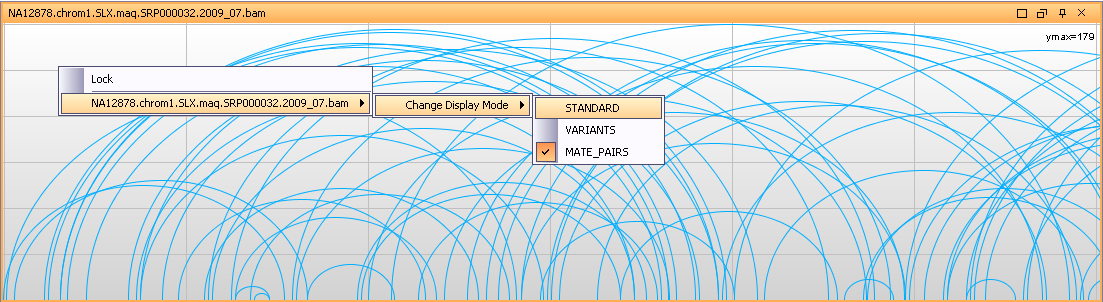
\includegraphics[type=png,ext=.png,read=.png,width=16cm]{images/changevizmode}
\caption{Changing the visualization mode.}
\label{changevizmode}
\end{center}
\end{figure*}

\chapter{Docking Framework}

Savant features a docking framework which allows users to rearrange modules to their liking. Such modules include tracks and built-in items (e.g. Bookmark, Table View, etc.) and plugins. Non-track modules are constrained to be docked to the sides of the UI and not among tracks. Similarly, track modules are constrained so that they cannot be docked among other modules.

While a number of important functions are presented here, the best way to learn all the features of the docking framework is to try using it.

\begin{figure*}[!h]
\begin{center}
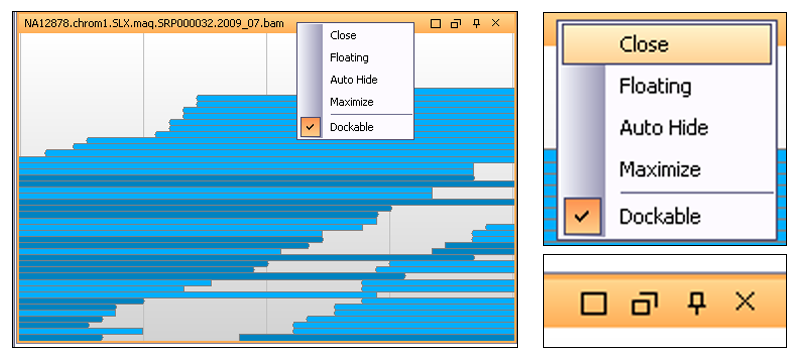
\includegraphics[type=png,ext=.png,read=.png,width=12cm]{images/dockingcontrols}
\caption{Left: A track module. Upper-right: Docking menu presented when the title bar of a module is right-clicked. Bottom-right: Docking controls embedded in the title bar of the module. The latter controls are {\it not} available in the Mac version.}
\end{center}
\end{figure*}

\section{Showing, hiding, and pinning modules}

By default, built-in modules are hidden. Hidden modules appear as tabs located on the region of the UI to which they are docked. A module is shown once the mouse is held over the tab. The shown module will hide once the mouse leaves the tab and focus is returned to another component of the UI. To force the module to be shown always, it can be "pinned". On Windows and Linux, a module can be pinned by pressing the pin icon located on the title bar of the module, making the pin point downwards. A pinned module can be hidden again by pressing the pin again, making the pin point to the left. On a Mac, a module can be pinned by first right-clicking the title bar of the module, then unchecking "Auto-hide". A pinned module can be hidden again by right-clicking the title bar of the module and checking "Auto-hide". The same functionality is possible through the title bar on Windows and Linux.

\begin{figure*}[!h]
\begin{center}
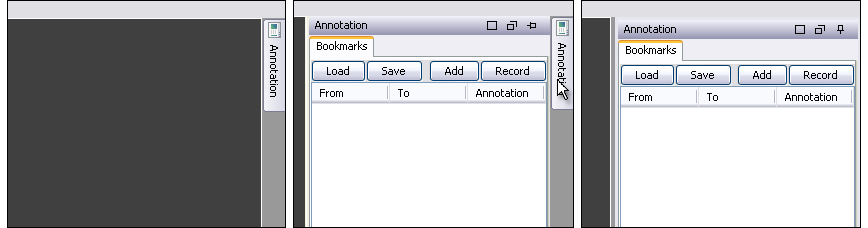
\includegraphics[type=png,ext=.png,read=.png,width=14cm]{images/hideshowmodules}
\caption{Hiding and showing modules. Left: The Annotation module, hidden on the right of the Savant UI. Middle: The Annotation module, shown by mousing over the Annotation tab. Right: The Annotation module, pinned so that it will remain shown even when the user is interacting with other components of the UI. }
\label{rangecontrolpanel}
\end{center}
\end{figure*}

\section{Resizing Modules}

Modules can be resized. To resize a module, click an edge and drag it until it occupies the desired size. 

\section{Rearranging modules}

Modules can be arranged in virtually any configuration within the UI. To move a module, click its title bar and drag it to the desired new location. While dragging, a gray outline will appear showing the location the module will occupy if the mouse is released. Track modules can be docked to the top or bottom of the track space, while other modules can be docked to any edge of the UI. In addition, modules can be docked on top of each other (in which case tabs will appear allowing one to switch between modules) or beside each other.

\begin{figure*}[!h]
\begin{center}
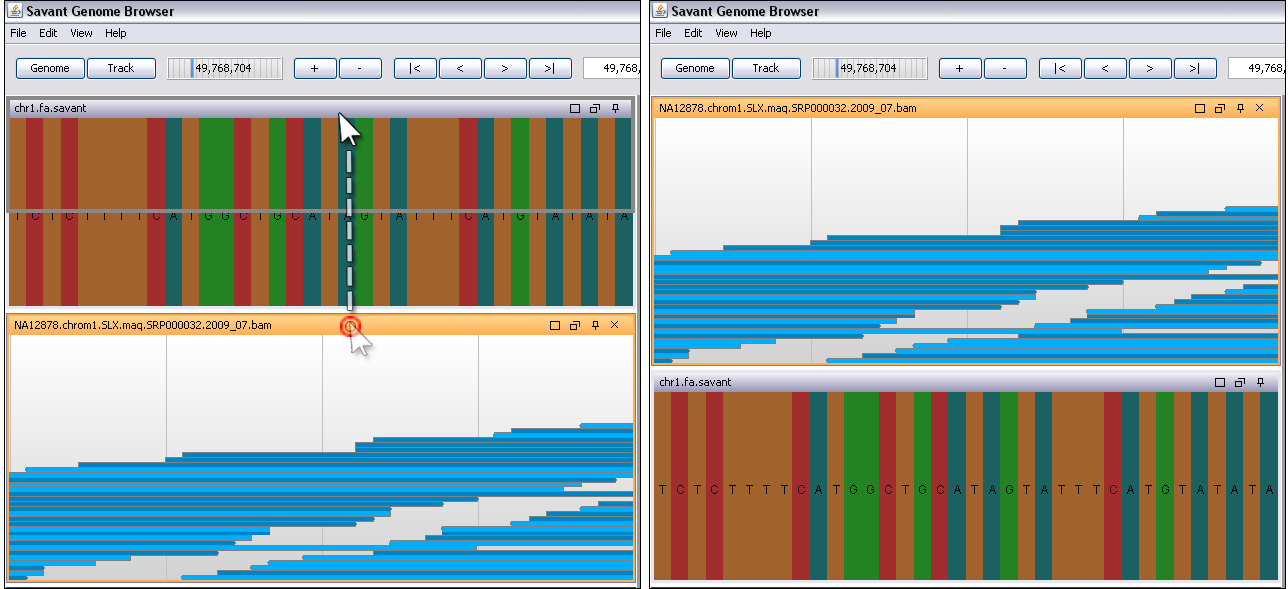
\includegraphics[type=png,ext=.png,read=.png,width=14cm]{images/arrangemodules}
\caption{Rearranging modules. Left: Demonstration of the rearrangement process. Right: The result of the rearrangement.  }
\label{rangecontrolpanel}
\end{center}
\end{figure*}

\section{Maximizing and restoring modules}

A module can be maximized to occupy the entire screen or UI, to make interaction or visualization with it easier, and then restored back to its original state among other modules to resume a concerted view. To maximize, press the embedded icon which resembles a square. To restore, press the embedded icon which resembles two overlapping squares (in the same location as the icon pressed to maximize). On a Mac, you can maximize and restore by right-clicking the title bar and click maximize and restore, respectively. The same functionality is possible through the title bar on Windows and Linux.

\section{Detaching and attaching from and to the UI}

A module can be detached from the UI and moved to a separate location on the screen. This is particularly useful for multidisplay setups where, for example, analytics modules can be moved to one display and tracks kept on another. To detach a module, press the embedded icon which resembles to squares. The detached module can then be moved to another location by clicking and dragging its title bar. To reattach it to the UI, press the embedded icon which resembles a square with an L-shape in it (in the same location as the icon pressed to detach it). On a Mac, you can detach and reattach by right-clicking the title bar and checking or unchecking Floating, respectively. The same functionality is possible through the title bar on Windows and Linux.


\chapter{Bookmarking}

The Bookmarks module helps to keep track of interesting regions or to make annotations. At any time, users may add, remove, or seek to a bookmarked region by using buttons within the module or by using keyboard shortcuts. 

\begin{figure*}[!h]
\begin{center}
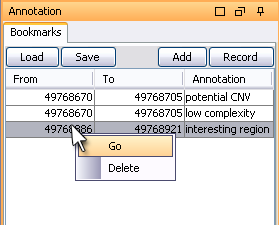
\includegraphics[type=png,ext=.png,read=.png,width=6cm]{images/bookmarks}
\caption{Bookmarks module.  }
\label{rangecontrolpanel}
\end{center}
\end{figure*}

\section{Adding and removing bookmarks}

A bookmark can be added by pressing the Add button embedded in the Bookmarks module. The current range will be used for the bookmark, although the from and to coordinates of the bookmark can be adjusted by double clicking and changing them. The keyboard shortcut CTRL+B (or CMD+B on a Mac) can be used to quickly add a bookmark. Bookmarks can be removed by right clicking them and choosing the Delete option.

\section{Seeking to a Bookmark}

A bookmark can be seeked to by right clicking it and choosing the Go option.

\section{Adding annotations to bookmarks}

An annotation can be added to a bookmark by double-clicking the Annotation field and typing in some text. 

\section{Recording Navigation History}

Navigation history can be tracked by clicking the Record button embedded in the Bookmarks module. From then on, every new range viewed will be stored as a Bookmark. To stop recording, press the Stop Recording button.

\section{Saving and loading bookmarks}

Bookmarks can be saved, to be reused in future sessions or to be shared with colleagues. To save the existing bookmarks, click the Save button embedded in the module. These bookmarks can subsequently be loaded by clicking the Load button embedded in the module. A user can opt to append the loaded bookmarks to the existing bookmarks, or to replace the existing bookmarks entirely with the loaded ones.

\chapter{Table View}

The Table View module displays the data in the current range in a tabular format. This module displays records as rows and fields as columns
in a spreadsheet. The data is automatically updated when a range is changed, unless the Auto Update checkbox is unchecked.

\begin{figure*}[!h]
\begin{center}
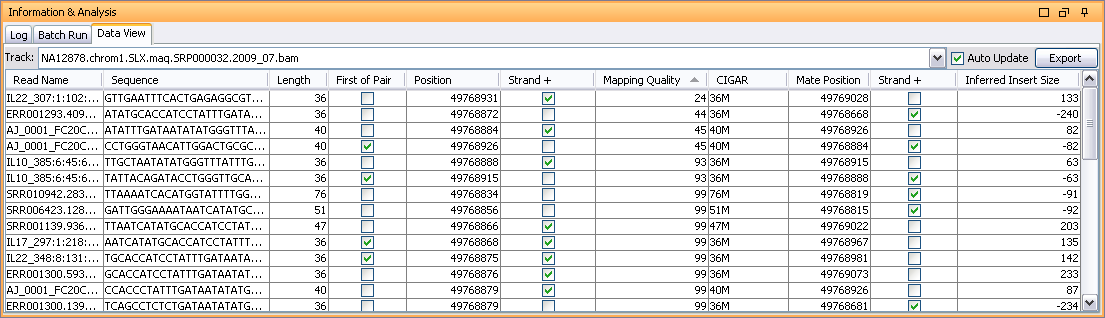
\includegraphics[type=png,ext=.png,read=.png,width=16cm]{images/tableview}
\caption{Table View module, showing data from a read alignment track.}
\label{rangecontrolpanel}
\end{center}
\end{figure*}

\section{Changing tracks}

The Table View only displays data from a single track at a time. To change the track whose data is being displayed, a drop-down list of tracks is provided from which to chose from.

\section{Sorting rows}

The entries in the Table View can be sorted by clicking the field header by which the rows are to be sorted.

\section{Exporting Data}

The data in the Table View can be exported by clicking the Export button embedded in the module. The resulting file is a tab-delimited encoding of the information shown in the browser.

\chapter{Plugins}

Savant is able to integrate plugins, allowing for powerful extensions of the browser. To learn how to develop a plugin, see the {\bf Developer's Guide} downloadable from the Savant website.

\section{Installing a plugin}

To install a third-party plugin, copy the plugin's .jar file to the Savant/plugins directory and restart Savant.

\section{Un-installing a plugin}

To un-install a third-party plugin, remove the plugin's .jar file from the Savant/plugins directory and restart Savant. Do not remove the SavantCore.jar file at any time.

\section{Using a plugin}

Every plugin works differently and may or may not have a user interface. For instructions on how to use a third-party plugin, see the developer's documentation.

\chapter{Other Features}

\section{Track Locking}

Individual tracks can also be locked to a particular range so that they are not updated until they are unlocked. Locked tracks can be used as overview profiles from which subregions can be selected to specify range changes for other tracks. To lock a track, right-click inside the track module and check the Lock option. While a track is locked, users may select a subrange from the track (by using the mouse zoom options, described previously) which will become the new range for other, unlocked tracks. To unlock a track, right-click inside the track module and uncheck the Lock option.

\end{document}
